%!TEX root = ../../thesis.tex

\section{Application to {CARMENES} spectra}

One of the main reasons for focusing on extending the work of~\citet{figueira_radial_2016} was to analyse the differences in {RV} precision of synthetic spectra and observed \nir{}.
This is important for the community to understand the accuracy of synthetic spectra.
\citet{artigau_optical_2018} recently found band-specific discrepancies in the theoretical precision between real and synthetic \nir{} spectra of Barnard's Star.
In 2018 {CARMENES} openly released a spectral library containing one spectrum for each target in their 324 M-dwarf {RV} survey in~\citet{reiners_carmenes_2018}.
With this they provide details on the empirical \(\delta V_{rms}\) measured during their {RV} processing with their {RV} analysis code, {SERVAL} \citep{zechmeister_spectrum_2018}, using all available spectra of each target.
Spectra from this library has been used to compare the theoretical precision of observed {CARMENES} spectra to synthetic models, and is still in the preliminary stages, with the progress so far demonstrated here.

\subsection{Target selection}
\label{subsec:carmense_targets}
To analyse the precision in different spectral types, a few specific M-dwarfs were selected.
These were selected from the 324 spectra of the {CARMENES} M-dwarf library from \citet{reiners_carmenes_2018} available at \href{http://carmenes.cab.inta-csic.es/gto/}{http://carmenes.cab.inta-csic.es/gto/}, along with the achieved \snr{} in the visible and \nir{} spectra.

The spectral library data was downloaded, divided into spectral type and ordered by the stated \nir{} {SNR}, to select targets at the high \snr{} end.
To cover the M-dwarf range, targets were selected near each of the spectral types M0, M3, M6 and M9.
For each spectral type (within $\pm0.5$) two stars are selected that have high {SNR} values. This will give eight spectra over the M-dwarf range to analysis.
One of the two selected targets for the M3 type is Barnard's star which has been analysed extensively in~\citet{artigau_optical_2018}, in particular with CRIRES spectra for the \nir{} domain, allowing for direct comparisons between the two works.
The other criteria used for selection was to select targets with a varied range of \Logg{} and \feh{} values if possible.

The selected targets from the {CARMENES} library are provided in \cref{tab:carmenes_selection_updated}.
The spectral parameters (\Teff{}, \Logg{}, \feh{}) for these targets are from \citet{passegger_carmenes_2018, rajpurohit_exploring_2018} who performed spectral fits of the {CARMENES} spectra with the {PHOENIX-ACES} and {BT-Settl} models respectively.
The uncertainties in the \citet{rajpurohit_exploring_2018} parameters are \(\sigma_{\teff{}}\)=100\K{}, \(\sigma_{\logg{}}\)=0.3, and \(\sigma_{\feh{}}\)=0.3 while the uncertainties on the 
\citet{passegger_carmenes_2018} values are \(\sigma_{\teff{}}\)=51\K{}, \(\sigma_{\logg{}}\)=0.07, and \(\sigma_{\feh{}}\)=0.16.
There are gaps in the \citet{passegger_carmenes_2018} values for stars that have the lower \snr{} levels as they are more difficult to analyse/fit.
Neither one has parameters for Luyten's Star, for which the parameters given are from {SIMBAD}.

\begin{landscape}
    %!TEX root = ../../thesis.tex

\begin{table}[h]
    \centering
    \begin{threeparttable}
        \caption[{CARMENES} targets for {RV} precision analysis.]{Selected {CARMENES} targets with stellar parameters from both~\citet{rajpurohit_exploring_2018} and~\citet{passegger_carmenes_2018}.}
        \begin{tabular}{lllcccccccc}
            %\small
            \toprule
            & & & & & \multicolumn{3}{c}{\citet{rajpurohit_exploring_2018}} & \multicolumn{3}{c}{\citet{passegger_carmenes_2018}} \\
            Karmn & Name & SpT & V & \(\snr{}_{\nir{}}\) & \Teff{} & \Logg{} & \feh{} & \Teff{} & \Logg{} & \feh{} \\
            &  &  & mag &  & \K{} & \si{\centi\metre\per\second\squared} & & \K{} & \si{\centi\metre\per\second\squared} &  \\
            \midrule
            J20533+621 & BD+61 2068     & M0.5 & 8.6  & 257 & 3900          & 5.5 & -0.5           & 3828 & 4.71 & 0.03 \\
            J04290+219 & BD+21 652      & M0.5 & 8.3  & 212 & 4000          & 5.5 & 0.5            & 4194 & 4.59 & 0.20 \\
            J07274+052 & Luyten's Star  & M3.5 & 9.9  & 254 & 3467\tnote{a} & -   & -0.1\tnote{a}  & -    & -    & -    \\
            J17578+046 & Barnard's Star & M3.5 & 9.5  & 236 & 3400          & 5.5 & 0.1            & 3278 & 5.10 & -0.12 \\
            J11055+435 & WX UMa         & M5.5 & 14.5 & 140 & 3000          & 5.5 & 0.3 & - & - & - \\
            J10564+070 & CN Leo         & M6.0 & 13.5 & 133 & 2900          & 5.4 & 0.1 & - & - & - \\
            J18356+329 & LSR J1835+3259 & M8.5 & 18.3 & 50  & 2400          & 5.0 &-0.1 & - & - & - \\
            J04198+425 & LSR J0419+4233 & M8.5 & 11.1 & 42  & 2400          & 4.9 & 0.1 & - & - & - \\
        \bottomrule
        \end{tabular}\label{tab:carmenes_selection_updated}
        \begin{tablenotes}
            \item [a] {From SIMBAD.}
        \end{tablenotes}
    \end{threeparttable}
\end{table}

\end{landscape}


\subsubsection{Spectral preparation and Telluric correction}
\label{subsec:prepatation_on_carmenes}
The spectra in the  {CARMENES} library have not been corrected for telluic lines.
To properly assess the theoretical {RV} precision attainable in the {CARMENES} spectra they need to be corrected for telluic lines.
Telluric correction is performed with the {Molecfit} software~\citep{smette_molecfit_2015} in collaboration with Sol\'ene Ulmer-moll, who has {Molecfit} experience~\citep{ulmer-moll_telluric_2018}.

The separate spectral orders first need to be combined into a single spectrum.
At this stage, where spectral orders overlap only the flux from one order is kept for simplicity.
The overlapping regions could be combined by taking the mean because the overlapping orders are well aligned in wavelength, but this was not performed at this exploratory stage.

The telluric correction is performed by dividing the {CARMENES} spectrum by a telluric transmission spectrum fitted with {Molecfit}.
The fitting with {Molecfit} has been attempted two different ways.
The first correction performs the fitting on the full \nir{} spectrum, while the second splits the spectrum into three parts and fits them separately.
This was done because it was noticed that the spectral line shape changes significantly from 0.9\um{} to 1.7\um{}.

Different molecules are fitted in the three separate parts.
In the first part (0.9--1.1\um{}) \ce{H2O} is fitted, in the second (1.1--1.5\um{}) \ce{O2} is fitted while \ce{CO2} and \ce{CH4} are fitted in the third section (1.5--1.71\um{}).
After this all molecule abundances are fixed and the final fit is performed on each of the three parts.

In the end, splitting the spectrum into three does not seem to improve the telluric correction considerably.
The telluric spectrum fitted from both attempts is shown in the top panel of \cref{fig:compare_telluric_corrections}.
The difference between the two telluric spectra changes is shown in the bottom panel.

It is unknown whether the full telluric correction of the {CARMENES} \nir{} spectrum has been performed before.
There has been one publication known which uses {Molecfit} to correct a {CARMENES} spectrum, but only in a very narrow spectral range (1.082--1.084\um{})~\citep{allart_spectrally_2018}.
As such there is not yet a definitive guide to achieve the best telluric correction of {CARMENES} spectra with {Molecfit}.

In this work only one spectrum has been telluric corrected to compare the difference between the two {Molecfit} corrections and their improvement over complete telluric masking on spectral quality and {RV} precision.
This was to see if it is worth investing time to improve the telluric correction step.

After telluric correction the spectrum was corrected for bad pixels by linear interpolation across them.
Some examples of bad pixels can be seen in a narrow wavelength range in \cref{fig:carmenes_spike_removal}.
The lines with orange circles and green crosses are the original and telluric corrected spectra, respectively.
They both show individual bad pixel spikes throughout the spectrum.
The black line is the spectrum corrected from the bad pixels (labelled `fixed') for the bad pixels. 
The blue line is a ``quality flag'' output (0 or 1) from {Molecfit}, indicating where the spectrum has a flux below or equal to zero.
It correctly identifies one of the bad pixels but not the others that have a flux above zero.
Within the \emph{Y}- \emph{J}-, and \emph{H}-bands there are around 213/66069\(\sim\)0.3\% bad pixels identified with an automated algorithm, based on a maximum derivative threshold (the bad pixels have very high derivatives).

The removal of bad pixels, which introduce pixels with very high derivatives (and pixel weight, $W(i)$), is essential for an accurate computation of the spectral quality and RV precision.
The sharp lines with high derivatives would artificially increases the calculated spectral quality, \(Q\), masquerading as very deep and narrow spectral lines.

\begin{figure}
    \centering
    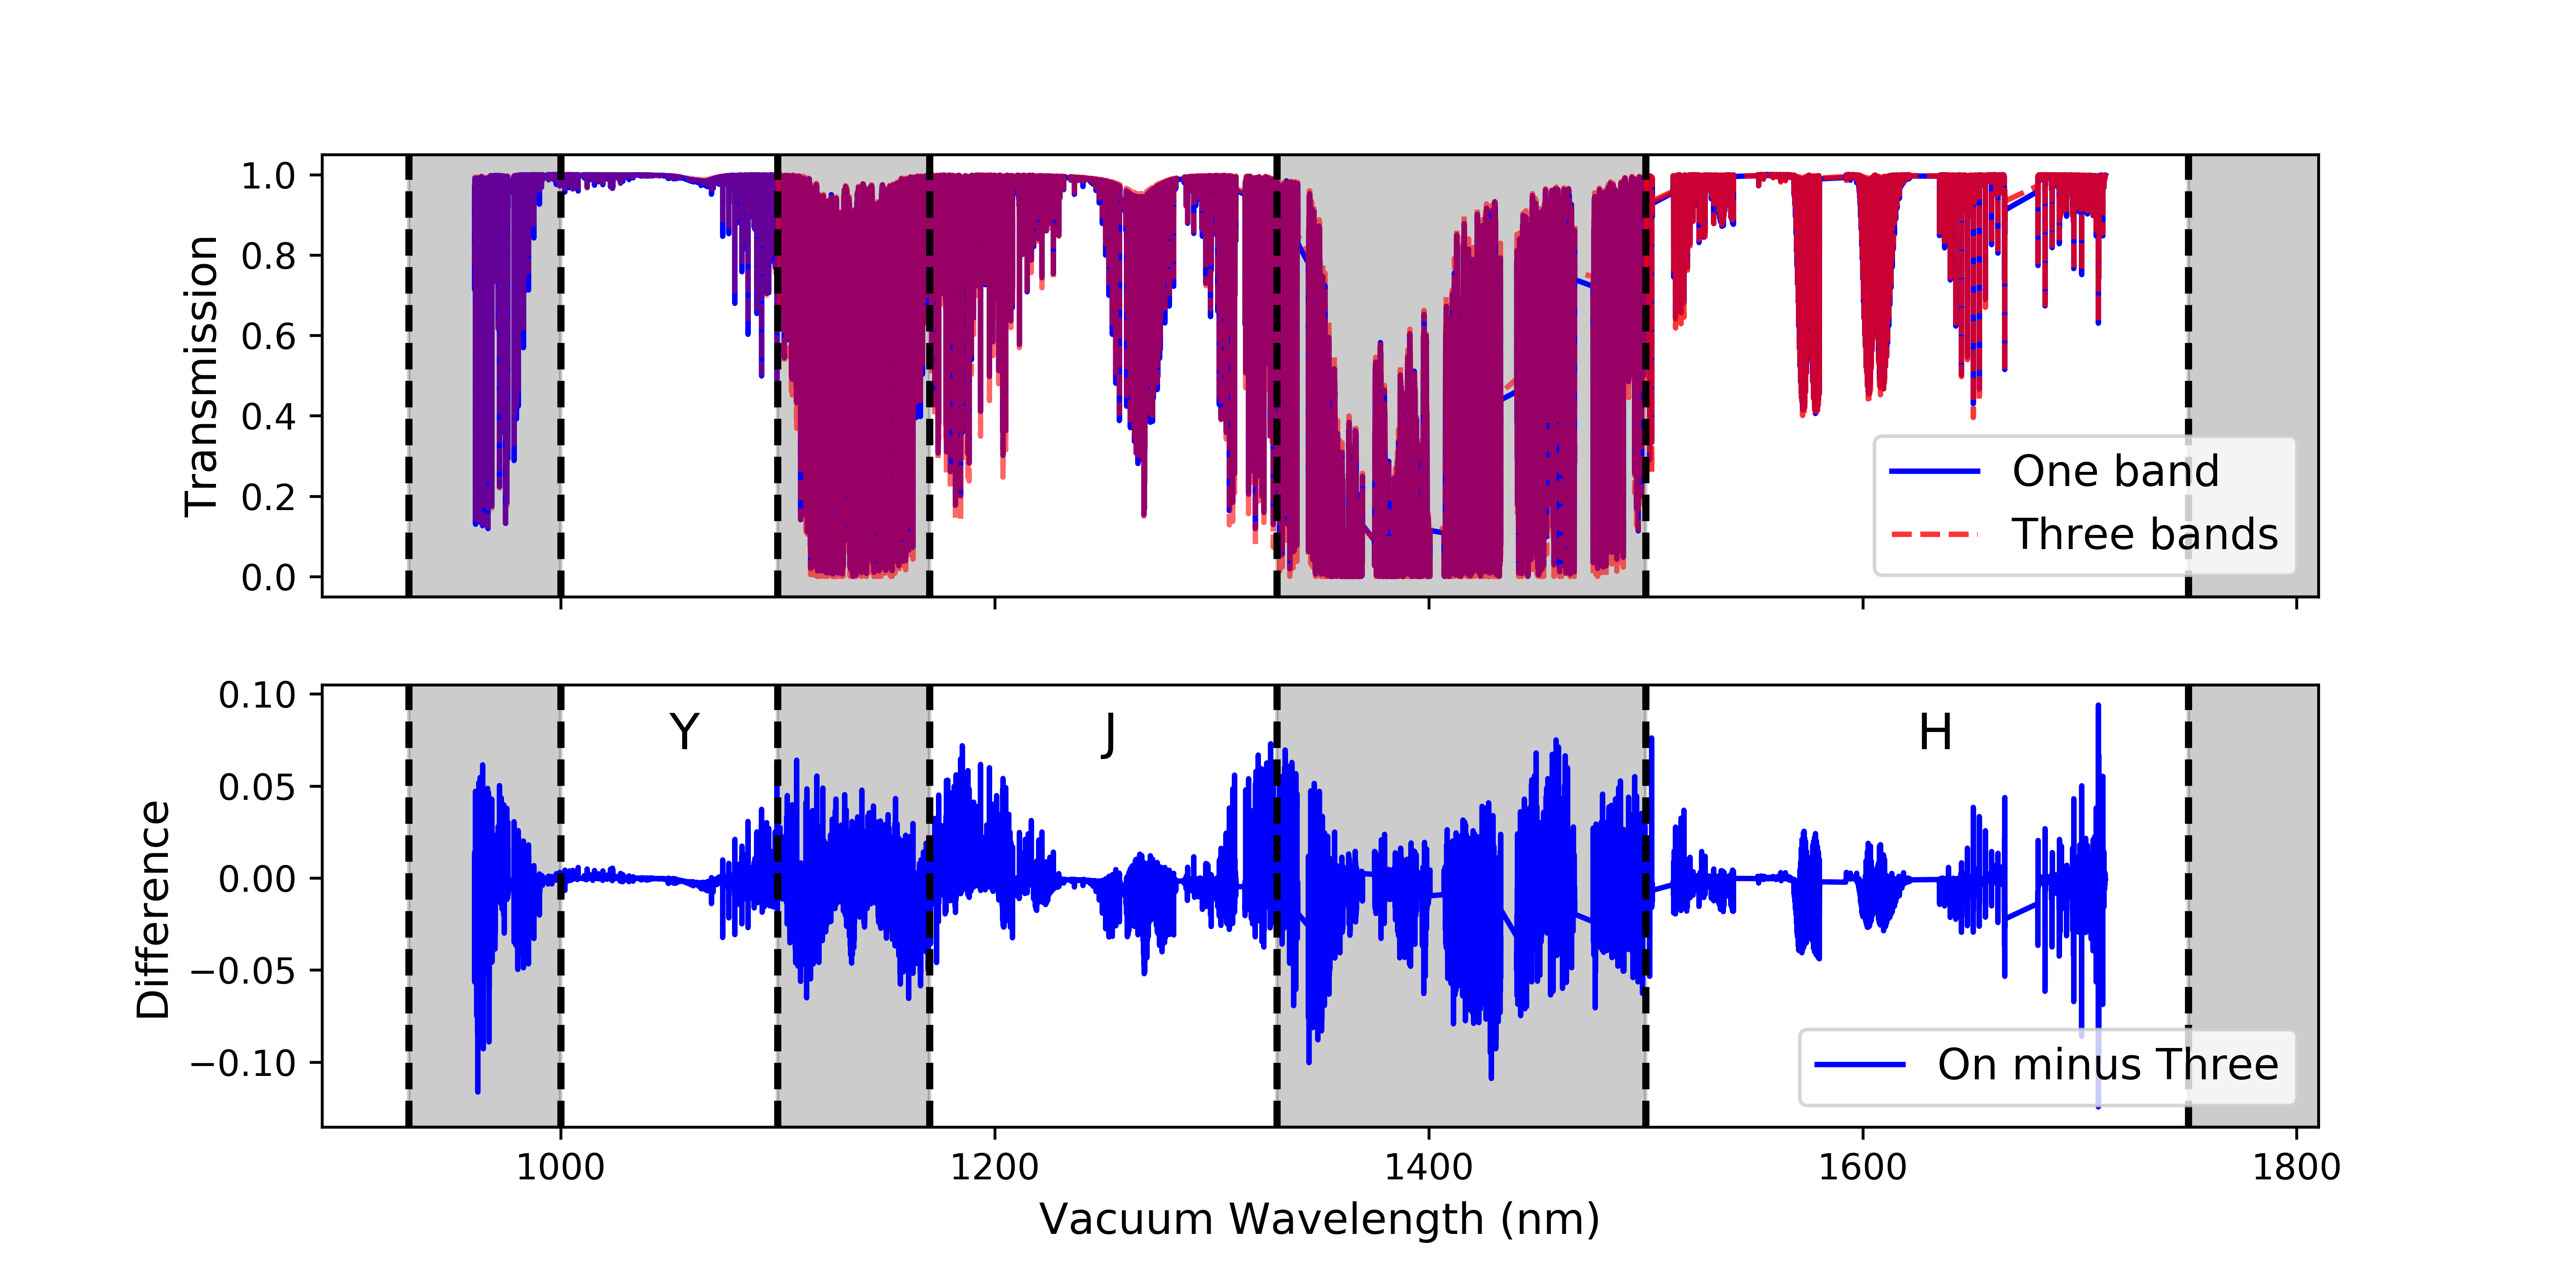
\includegraphics[width=0.9\linewidth]{figures/information-content/Carmenes/compare_telluric_corrections_shaded}
    \caption[]{Comparison of telluric models in pursuit of a better correction.
        Top: The two synthetic telluric spectra.
        The blue shows the result from {Molecfit} after treating the full spectrum as one, with a single spectral profile, while the shaded red telluric spectrum has been derived with three separate bands, fitted individually.
        Bottom: The difference in the telluric spectrum between the fit to the full spectrum, and the fit with the spectrum split into three.
        The regions of deep \ce{H2O} absorption lines which defined the \nir{} bands are shaded grey.
        The bounds of each band from \cref{tab:infrared_bands} are indicated with vertical black dashed lines.}
    \label{fig:compare_telluric_corrections}
\end{figure}


\begin{figure}
    \centering
    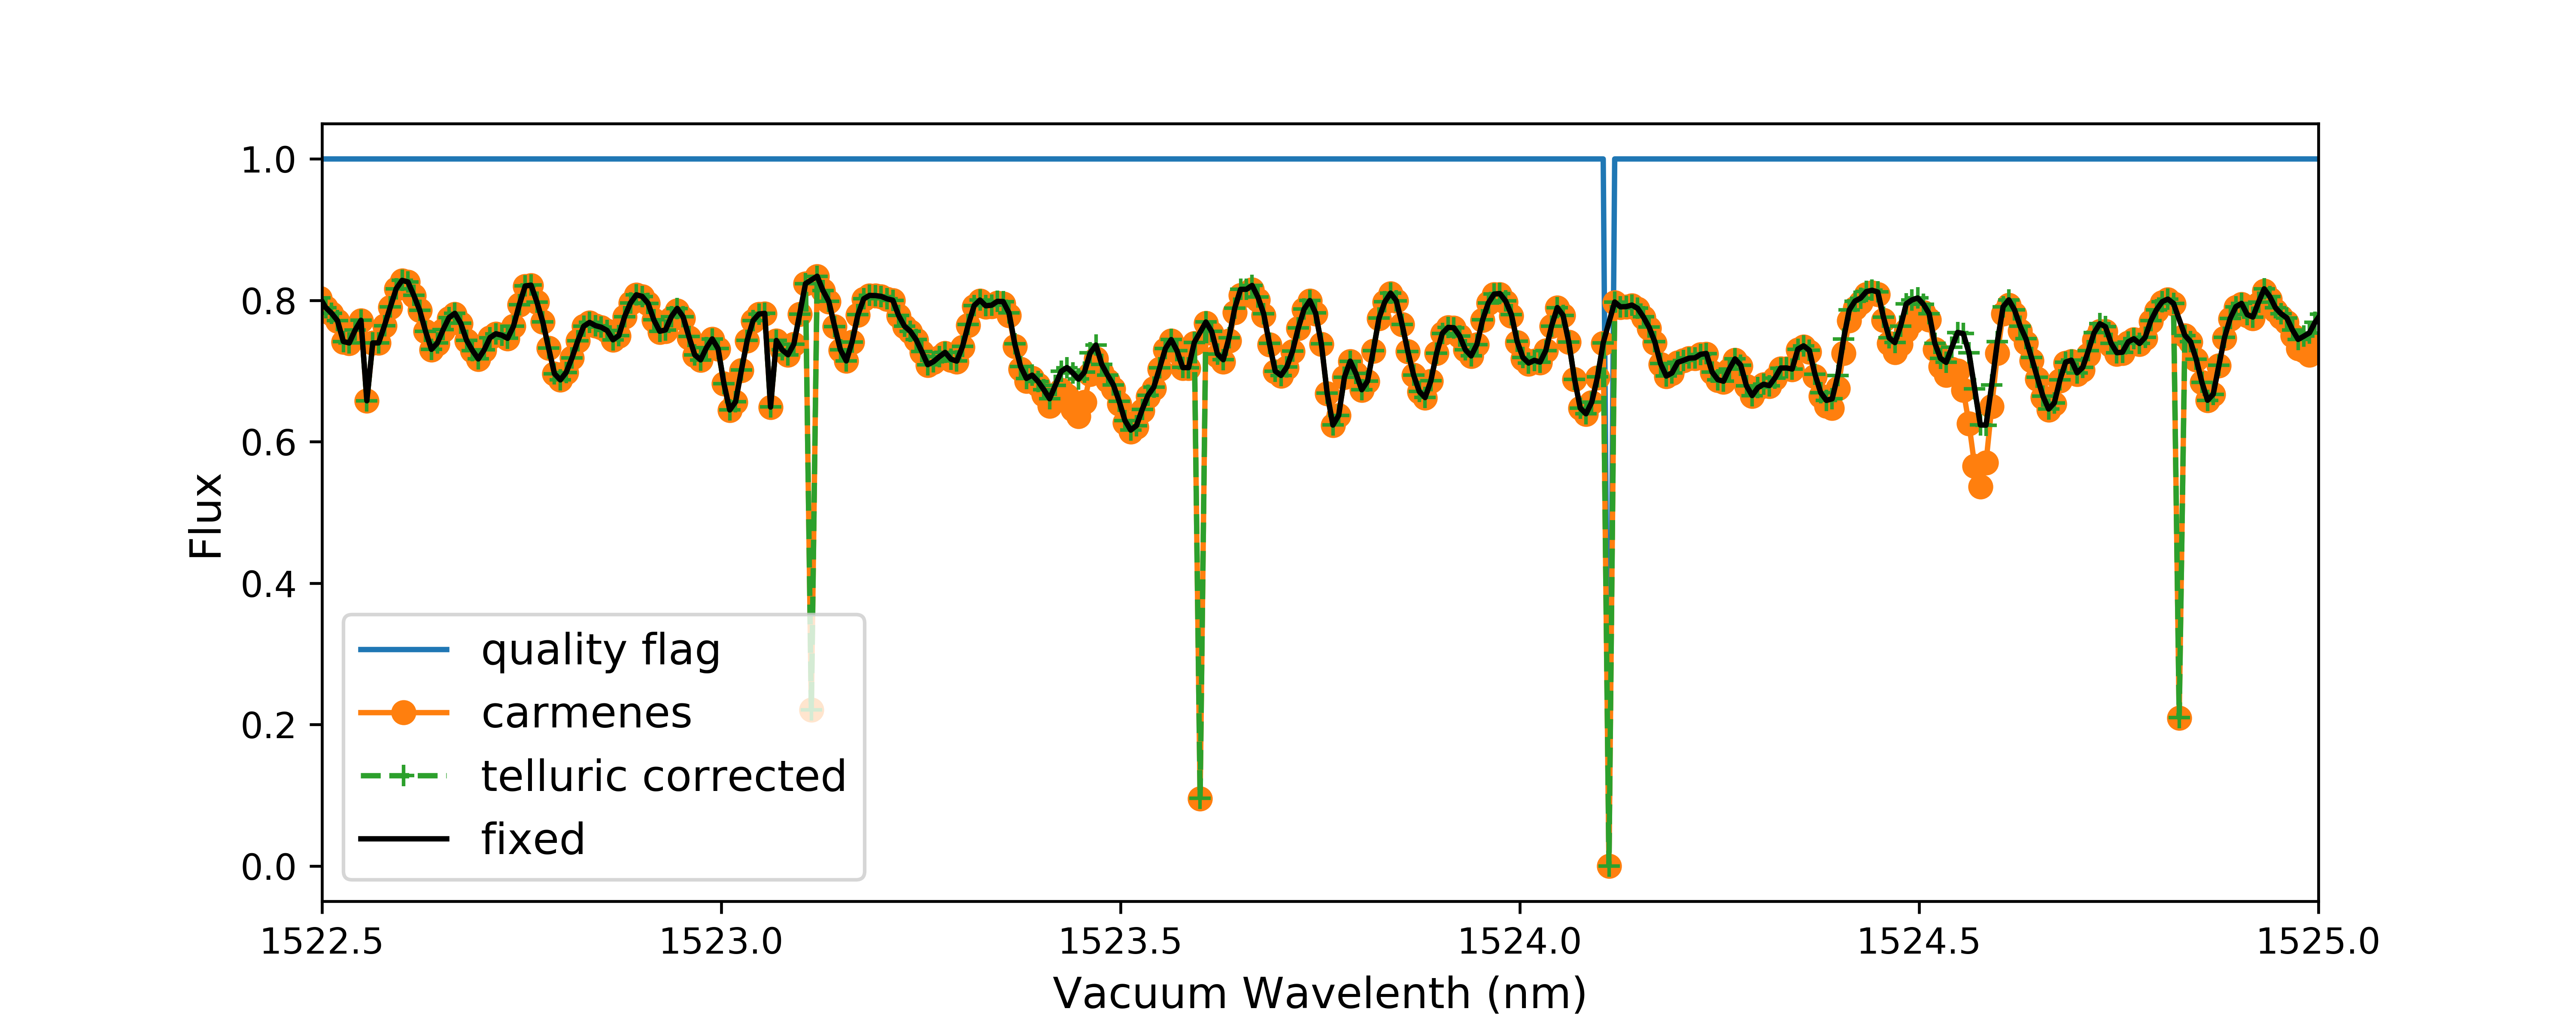
\includegraphics[width=0.9\linewidth]{figures/information-content/Carmenes/carmenes_spike_removal}
    \caption[Bad pixel removal in {CARMENES}.]{Removal of bad pixels from the {CARMENES} spectrum. The orange line with circles and green line with pluses are the original and telluric corrected spectra from {CARMENES}.
    The black solid line shows the spectrum after correction from bad pixels.
    The blue line shows the ``quality flag'' (0 or 1) output from the {Molecfit} software.}
    \label{fig:carmenes_spike_removal}
\end{figure}


\subsection{Impact of telluric correction}
\label{subsec:impact_telluric_correction}
Here the impact of the telluric correction on the spectral quality of the CARMENES spectrum is assessed.
This was done by calculating, Q, with the original telluric lines deeper than 2\% masked out, and with the telluric correction performed.
This was done for both fitting methods attempted with Molecfit and displayed in \cref{fig:band_qualityfromapplyingtelluriccorrection}.
The top panel shows the telluric corrected spectrum (orange) along with the telluric mask that was applied (blue).
The bottom panel shows the spectral quality for the three spectral bands \emph{Y}, \emph{J}, and \emph{H}.

\begin{figure}
    \centering
    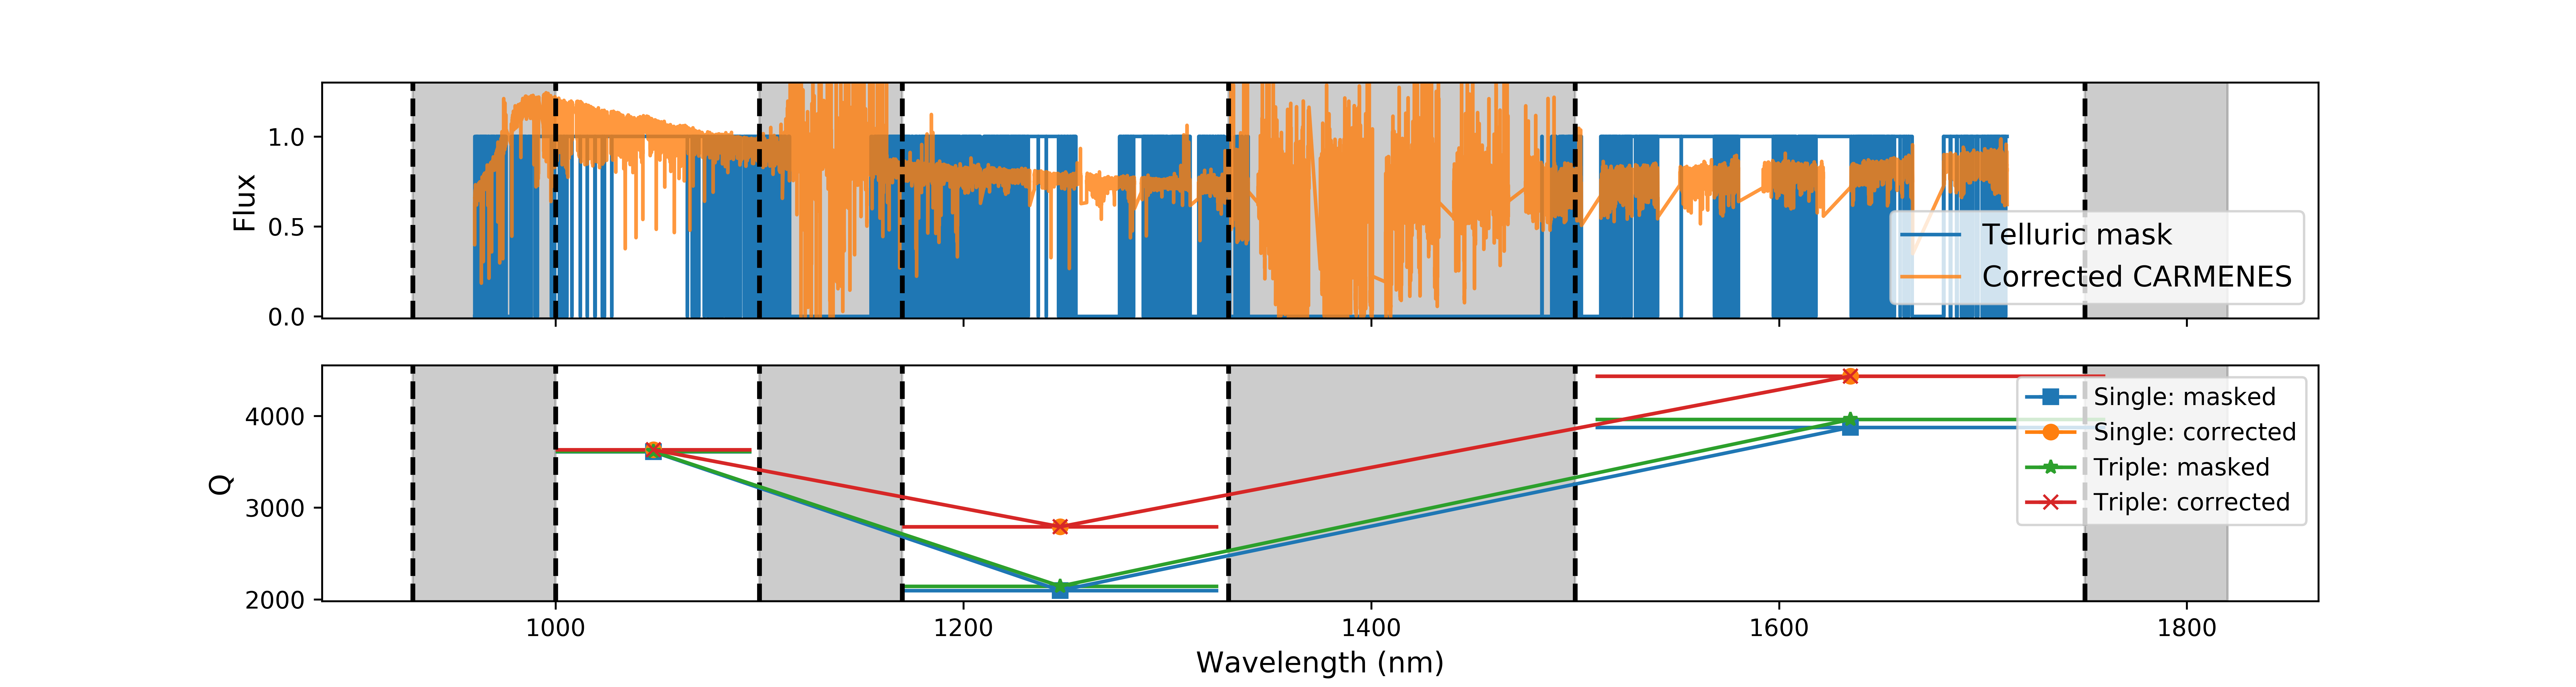
\includegraphics[width=0.8\linewidth]{figures/information-content/Carmenes/Band_quality_from_applying_telluric_correction}
    \caption[Barnard's star spectral quality.]{Measured spectral quality, Q, in the three \nir{} bands of Barnard's star to assess the gain from telluric correction. 
        Top: The telluric corrected CARMENES spectrum (orange) along with the binary mask for telluric lines >2\% depth (blue). 
        Bottom: The spectral quality in the three spectral bands, for different telluric treatment. `single' indicates the Molecfit results from the single fit to the spectrum, while `triple' indicates the fit to the three wavelength bands.
        `masked' indicates that telluric masking of the lines deeper than 2\% was performed and while `corrected' is just the telluric corrected spectrum.}
    \label{fig:band_qualityfromapplyingtelluriccorrection}
\end{figure}

\cref{fig:band_qualityfromapplyingtelluriccorrection} shows that there is a benefit (gain in quality) from telluric correction in the \emph{J} and \emph{H}-bands, where there are numerous telluric lines.
However, in the \emph{Y}-band where there is little telluric masking performed there is only a slight gain.
Performing telluric correction of the CARMENES spectra over telluric masking causes a gain the the spectral quality by 1\%, 30\%, 12\% in the \emph{Y}-band, \emph{J}, and \emph{H}-bands respectively.
As the spectral quality is related to the RV precision, this will lead to a 10-30\% improvement in the RV precision in the \emph{J}- and \emph{H}-bands
This indicated that it is worth performing telluric correction on the other seven {CARMENES} targets selected.
This also shows that the extra effort from three separate telluric fittings does not lead to a significant gain in quality.


\subsection{Barnard's star}
\label{sec:carmenes_barnards_star}
Currently only Barnard's star has had the telluric correction performed, and as such the analysis for this target is shown.
The spectral content of Barnard's star was extensively explored in \citet{artigau_optical_2018} comparing the synthetic model to observations from {HARPS}, {ESPaDOns} and {CRIRES} in the range 380--2300\nm{}.
Agreement was found in the optical but the \nir{} bands had significant differences between the observations and models. 
The goal of this analysis is to check if the same results are obtainable in the {CARMENES} spectrum of Barnard's star.

\citep{artigau_optical_2018} tabulated several literature values for the stellar properties of Barnard's star and identified the closest matching {PHOENIX-ACES} model.
The synthetic model adopted for Barnard's star is \Teff=3200\K{}, \Logg{}=5.0, and \feh{}=-0.5.
This same model was adopted here.
This is tabulated in with other parameters from \citet{artigau_optical_2018} in \cref{tab:barnards_star_params}.

\begin{table}
    \centering
    \caption{Properties of Barnard's star from \citep{artigau_optical_2018}. \Teff{}, \feh{} and \Logg{} values are only the adopted (closest) model parameters.}
    \begin{tabular}{lc}
        \toprule
        Parameter & Value \\
        \midrule
        SpType & M4\,Ve \\
        Rotation Period & \(\sim\)130 days \\
        \Vsini{} & \(\le 80\) \si{\metre\per\second} \\
        \Teff{} & 3200 \K{} \\
        \Logg{} & 5.0 \\
        \feh{} & -0.5 \\
        \bottomrule{}
    \end{tabular}\label{tab:barnards_star_params}
\end{table}

A series of spectra are shown in \cref{fig:carmenes_correction}.
The uncorrected {CARMENES} spectrum of Barnard's Star is shown in the first panel.
The second panel shows telluric model from Molecfit, while the third panel shows the telluric corrected spectrum.
In the telluric corrected spectrum there are several deep spikes which are bad pixels.
Most of these are corrected for in the fourth panel, although it appears there may be a few still present in the spectrum.
The fifth panel contains the synthetic PHOENIX-ACES spectrum of Barnard's star, used to compare the spectral quality.
The model has been convolved by an instrumental profile with R=80\,400, but not rotationally broadened since the \Vsini{} is low. The flux units of the spectra are arbitrary, and the synthetic model has been converted into photon counts.


\begin{figure}
    \centering
    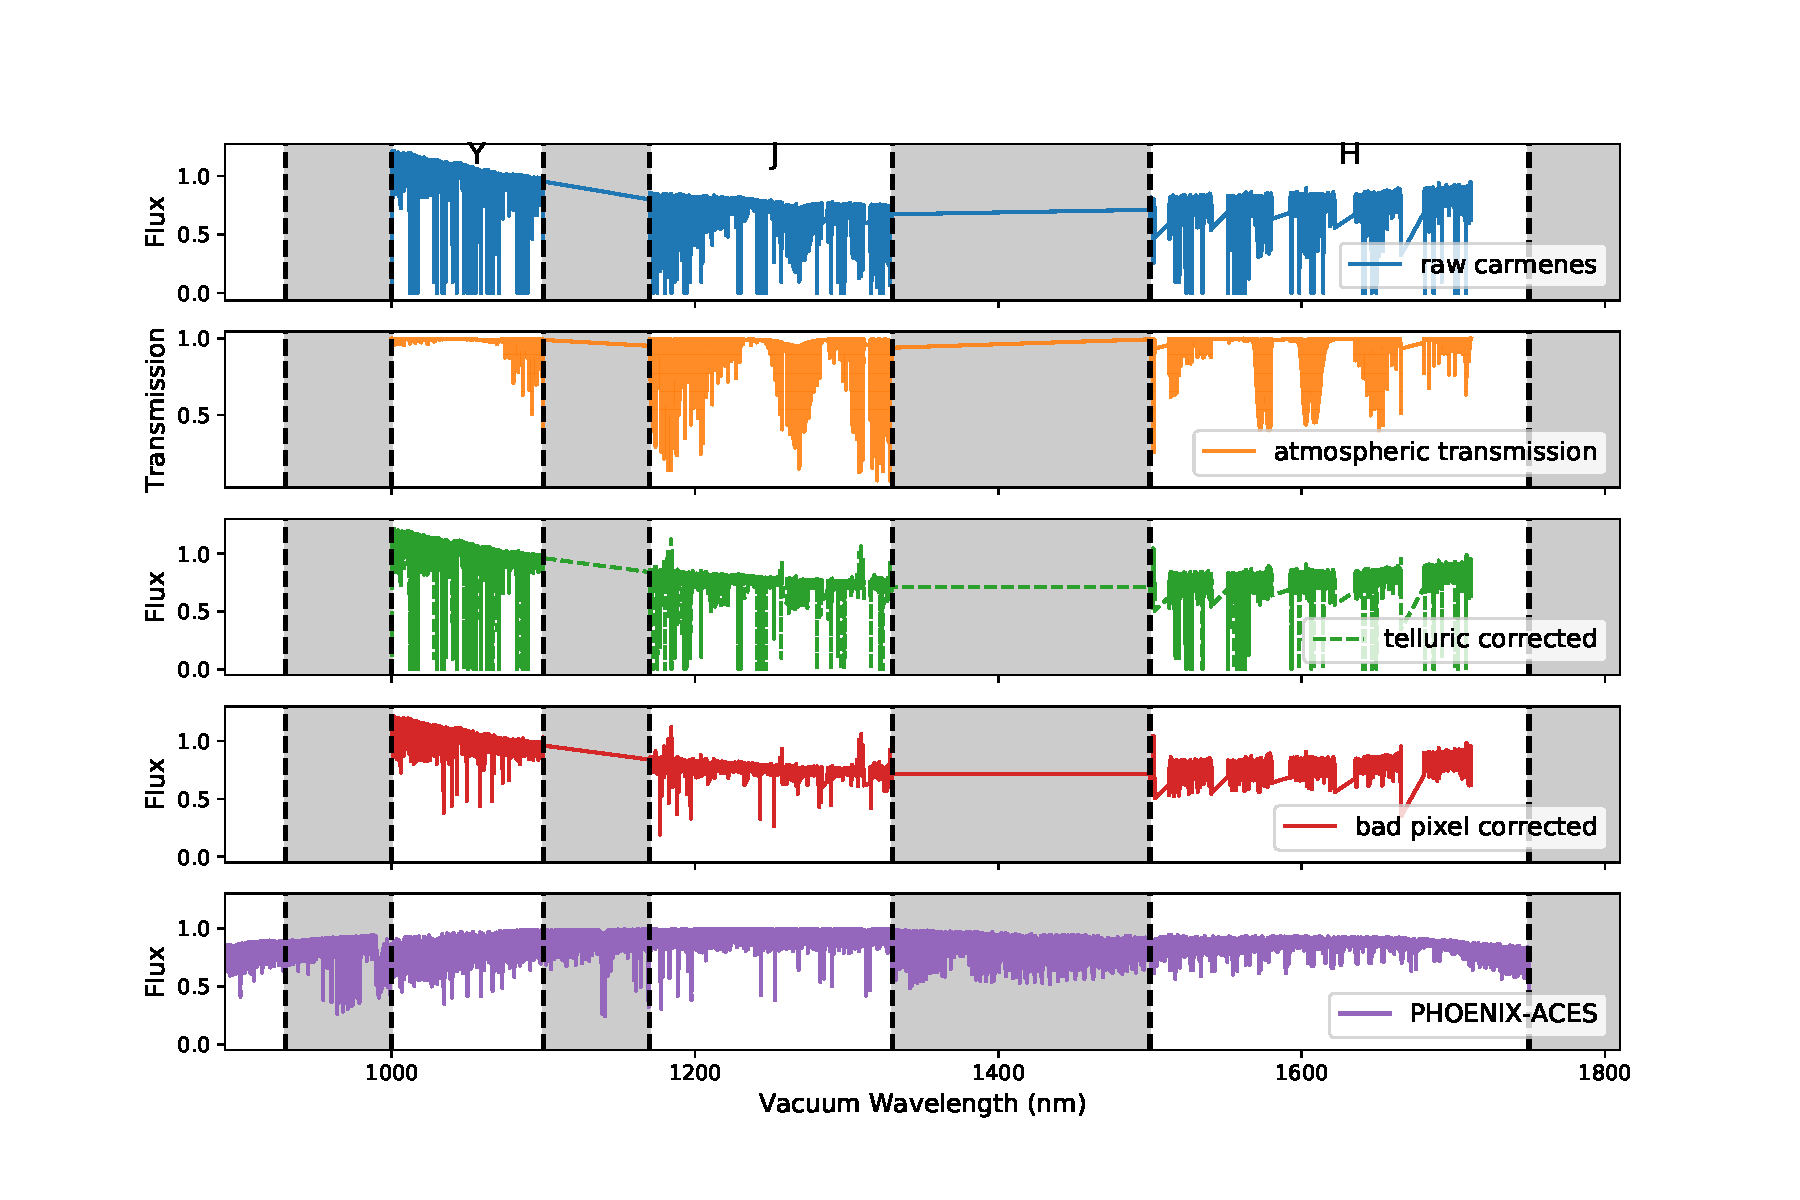
\includegraphics[width=0.8\linewidth]{figures/information-content/Carmenes/bp_carmenes_masked_model_broadened}
    \caption[Telluic correction of the {CARMENES} \nir{} spectrum.]{Telluic correction of the {CARMENES} \nir{} spectrum.
        First: Uncorrected spectrum of Barnard's Star between 960--1710\nm{} from {CARMENES}.
        Second: The synthetic telluric transmission spectrum fitted with {Molecfit}.
        Third: Telluric corrected spectrum by division of the telluric spectrum.
        The regions of deep \ce{H2O} absorption lines which defined the \nir{} bands are shaded grey.
        Fourth: The telluric corrected spectra after the bad pixels are removed.
        Fifth: Synthetic PHOENIX-ACES model for Barnard's star, convolved to R=80\,400.
        The bounds of each band from \cref{tab:infrared_bands} are indicated with vertical black dashed lines.
        The flux units of the spectra are arbitrary}
    \label{fig:carmenes_correction}
\end{figure}


To compare the model to the observation it is interpolated to the pixel positions of the {CARMENES} spectrum.
The spectral quality is calculated for both on small wavelength bins with a width 0.2\% the central wavelength similar to \citep{artigau_optical_2018}.
The top panel of \cref{fig:qualitycomparisiontomodel} shows the results of the comparison, with the spectral quality in 0.2\%\,\(\lambda\) width bins for the observation (orange squares) and the model (blue stars) in the top panel.
The ratio between the spectral quality of the observation and the model is given in the bottom panel.
It shows that in this instance the \emph{Y}- and \emph{J}-bands have a similar spectral quality, while there is a large difference in the \emph{H}-band with the CARMENES observation having a spectral quality 3--4\(\times\) greater than the model.

\begin{figure}
    \centering
    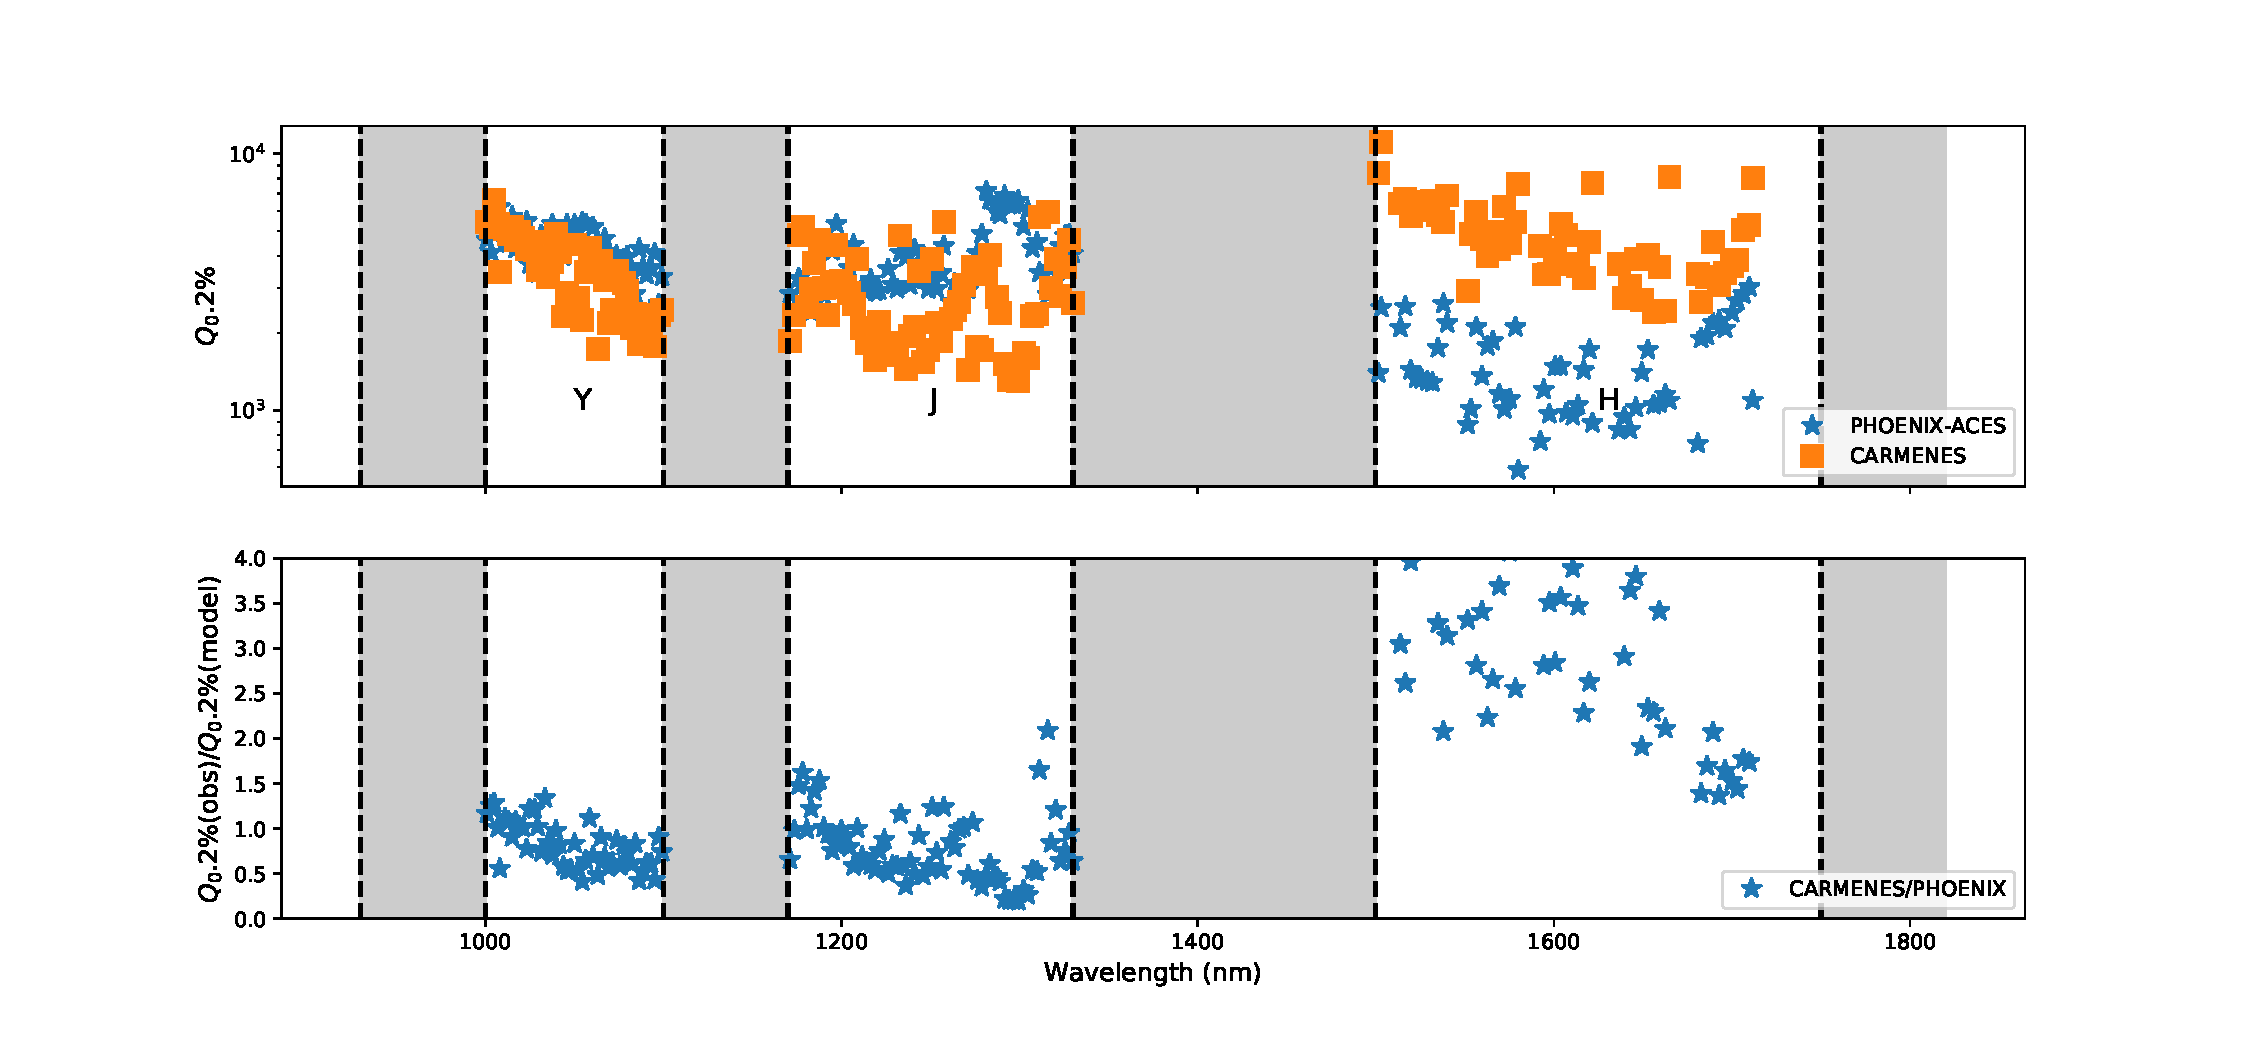
\includegraphics[width=0.8\linewidth]{figures/information-content/Carmenes/quality_comparision_to_model}
    \caption[Barnard's star spectral quality compared to CARMENES]{Measured RV content of Barnard's star over the near-infrared domain, from CARMENES.
    Top: The spectral quality in 0.2\%\,\(\lambda\) width bins for CARMENES (orange squares) and the model (blue stars).
    Bottom: The ratio of spectral quality observed/model.}
    \label{fig:qualitycomparisiontomodel}
\end{figure}

\cref{fig:allw2} from \citep{artigau_optical_2018} is shown for comparison.
In the \emph{Y}- and \emph{J}-bands \cref{arti} obtains a lower spectral quality (50\%) compared to the model.
However in this work the model and observation have a similar spectral quality in these bands, although the ratio does drop to 50\% in the latter apart of the \emph{J}.
In the \emph{H}-band of both works the observed quality is higher then the model, however the CARMENES spectral quality is 3\(\times\) higher, instead of only 1.5\(\times\) in \citep{artigau_optical_2018}.
This is a significant difference.

\citep{artigau_optical_2018} only apply telluric masking in their analysis, whereas here the telluric corrected spectra were used.
This could be part of the reason for the largely improved results in the \emph{H}.
As shown in \cref{subsec:impact_telluric_correction} the telluric correction can improve the quality by 12--30\%.
However, this does not fully explain the increase by a factor of 2.
This requires further investigation.


\begin{figure}
    \centering
    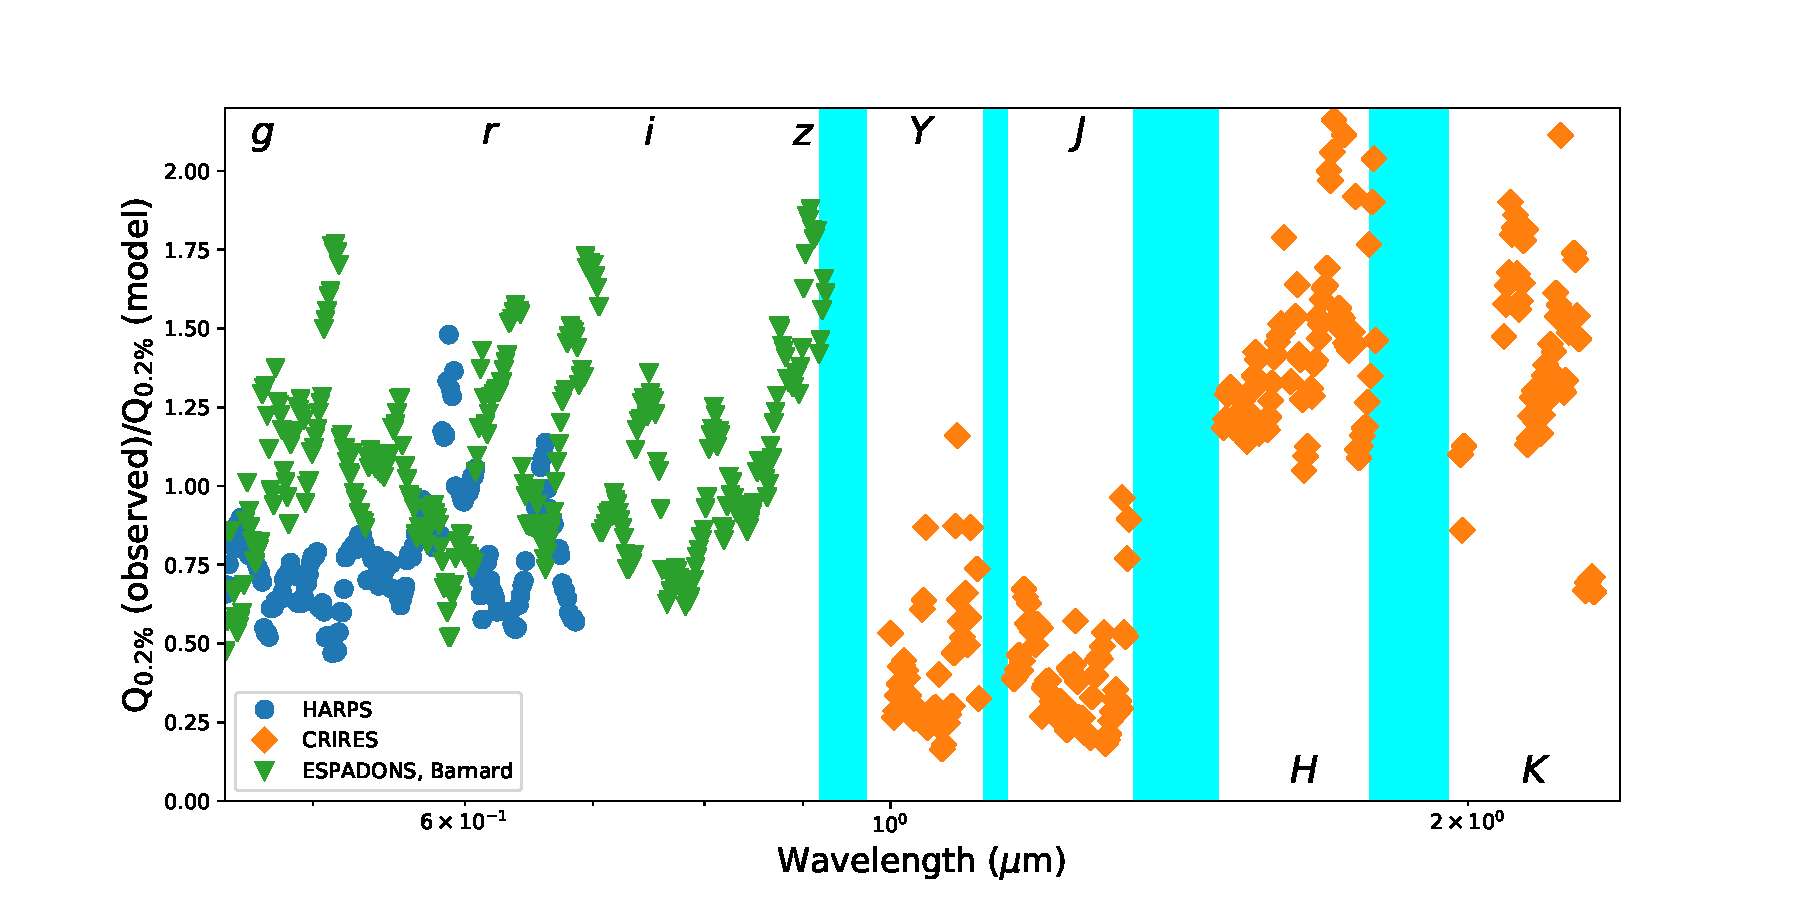
\includegraphics[width=0.8\linewidth]{figures/information-content/artigau2018_figures/all_w2}
    \caption[Measured RV content of Barnard's star over the optical and near-infrared domain.]{Measured RV content of Barnard's star over the optical and near-infrared domain. Overall measured (blue) and model (red) RV density are well matched blueward of $\sim1\mu$m. The agreement is poorer in the near-infrared domain with an over-prediction of RV content in $Y$ and \emph{J} bands and an under-prediction in \emph{H} and \emph{K}.
        Bottom: Ratio of observed to model $Q_{0.2\%}$ values. Areas unusable for RV measurements because of strong telluric absorption are filled in light blue. Reproduced from from \citep{artigau_optical_2018}.}
    \label{fig:allw2}
\end{figure}


%This work specifically added an extra feature to \eniric{} in the ability to calculate the precision on shorter wavelength scales rather than the full band. This is inspired and driven by the wavelength bins with a width \(2\%\times\lambda^\prime\), centred at \(\lambda^\prime\) as done in \citep{artigau_optical_2018}.
%This allows for a finer resolution of the spectral quality throughout the band rather than just the full band
%precision as done in \citet{figueira_radial_2016} and \cref{fig:band_qualityfromapplyingtelluriccorrection}.
%Analysis of the precision on smaller wavelength scales is also performed in other works~\citep[e.g.][]{bouchy_fundamental_2001, reiners_carmenes_2018}.


\subsubsection{Future tasks}
\label{subsubsec:future_tasksaims}
These results are still preliminary analyses, and a few things can be improved.
For instance the observed and model spectra have not yet been Doppler shifted to the same frame.
A Doppler shift of a few \nm{} is unlikely to affect the results shown in \cref{fig:qualitycomparisiontomodel} significantly.
There are also a few bad pixels that are still present in the observation that should be properly removed.

Adding the analysis of several CARMENES spectra across the M-dwarf range would be an important addition to this work to see if these results are consistent for all spectra, or if they are dependant on the stellar parameters.
